\documentclass[UTF8,a4paper,12pt]{ctexart}

% 加载报告排版宏包
\usepackage[left=2.6cm,right=2.6cm,top=2.6cm,bottom=2.6cm,headheight=15pt]{geometry}
\usepackage{setspace}
\usepackage{graphicx}
\usepackage{subcaption}
\usepackage{float}
\usepackage{booktabs}
\usepackage{tabularx}
\usepackage{array}
\usepackage{multirow}
\usepackage{enumitem}
\usepackage{amsmath}
\usepackage{amssymb}
\usepackage{xcolor}
\usepackage{tikz}
\usepackage{caption}
\usepackage{fancyhdr}
\usepackage{tocloft}
\usepackage{hyperref}

% 加载流程图组件
\usetikzlibrary{arrows.meta,positioning,calc,shapes.geometric}

% 设置图片路径
\graphicspath{{figures/}}

% 设置超链接样式
\hypersetup{
  colorlinks=true,
  linkcolor=black,
  urlcolor=black,
  citecolor=black
}

% 设置正文格式
\onehalfspacing
\zihao{-4}
\setlength{\parindent}{2em}
\setlength{\parskip}{0pt}
\setlist{nosep,leftmargin=2.5em}

% 设置章节标题格式
\ctexset{
  section={
    format={\centering\heiti\zihao{3}},
    name={,},
    number=\arabic{section},
    aftername=\quad,
    beforeskip=1.2em,
    afterskip=1.0em
  },
  subsection={
    format={\heiti\zihao{4}},
    name={,},
    number=\arabic{section}.\arabic{subsection},
    aftername=\quad,
    beforeskip=0.8em,
    afterskip=0.4em
  },
  subsubsection={
    format={\heiti\zihao{-4}},
    name={,},
    number=\arabic{section}.\arabic{subsection}.\arabic{subsubsection},
    aftername=\quad,
    beforeskip=0.5em,
    afterskip=0.2em
  }
}

% 设置目录格式
\renewcommand{\contentsname}{\zihao{3}\heiti 目\quad 录}
\renewcommand{\cfttoctitlefont}{\hfill\zihao{3}\heiti}
\renewcommand{\cftaftertoctitle}{\hfill}
\renewcommand{\cftsecfont}{\songti\zihao{-4}}
\renewcommand{\cftsubsecfont}{\songti\zihao{-4}}
\renewcommand{\cftsecpagefont}{\songti\zihao{-4}\mdseries}
\renewcommand{\cftsubsecpagefont}{\songti\zihao{-4}\mdseries}
\renewcommand{\cftsecleader}{\cftdotfill{\cftdotsep}}
\setlength{\cftbeforetoctitleskip}{0pt}
\setlength{\cftaftertoctitleskip}{0.8em}
\setlength{\cftbeforesecskip}{0.45em}
\setlength{\cftbeforesubsecskip}{0.15em}
\cftsetindents{section}{0em}{2.2em}
\cftsetindents{subsection}{2.0em}{3.0em}

% 设置图表格式
\renewcommand{\figurename}{图}
\renewcommand{\tablename}{表}
\captionsetup{font=small,labelfont=bf,labelsep=quad,justification=centering}
\numberwithin{figure}{section}
\numberwithin{table}{section}
\renewcommand{\thefigure}{\thesection-\arabic{figure}}
\renewcommand{\thetable}{\thesection-\arabic{table}}

% 设置页眉页脚
\pagestyle{fancy}
\fancyhf{}
\fancyhead[C]{\songti\zihao{-5}高频地波雷达目标跟踪技术总结报告}
\fancyfoot[C]{\songti\zihao{-5}\thepage}
\renewcommand{\headrulewidth}{0.4pt}
\renewcommand{\footrulewidth}{0pt}

\fancypagestyle{plain}{
  \fancyhf{}
  \fancyhead[C]{\songti\zihao{-5}高频地波雷达目标跟踪技术总结报告}
  \fancyfoot[C]{\songti\zihao{-5}\thepage}
  \renewcommand{\headrulewidth}{0.4pt}
  \renewcommand{\footrulewidth}{0pt}
}

% 定义流程图样式
\tikzset{
  block/.style={draw=blue!55!black,rounded corners=2pt,align=center,minimum height=0.85cm,minimum width=2.45cm,fill=blue!5,line width=0.6pt},
  data/.style={draw=teal!60!black,rounded corners=2pt,align=center,minimum height=0.85cm,minimum width=2.45cm,fill=teal!6,line width=0.6pt},
  judge/.style={draw=orange!70!black,rounded corners=2pt,align=center,minimum height=0.85cm,minimum width=2.45cm,fill=orange!8,line width=0.6pt},
  arrow/.style={-{Stealth[length=2.2mm]},thick,draw=black!75}
}

\begin{document}

% 生成目录页
\pagenumbering{Roman}
\thispagestyle{plain}
\tableofcontents

\newpage
\pagenumbering{arabic}
\setcounter{page}{1}

\section{高频地波雷达工作原理及特点总结}

\subsection{工作原理}

高频地波雷达通常工作在 3--30 MHz 频段。该频段电磁波能够沿导电海面发生绕射传播，因此可以突破普通微波雷达的视距限制，对远距离海域进行连续观测。雷达发射高频电磁波后，海面、船舶和环境散射体会产生回波。接收端经过混频、采样、距离向处理、速度向处理和方位向处理后，可得到距离、径向速度、方位角、幅度和信噪比等点迹信息。

距离观测由电磁波往返传播时间决定。设电磁波传播速度为 \(c\)，目标距离为 \(R\)，回波时延为 \(\tau\)，则有
\begin{equation}
  \tau = \frac{2R}{c},
  \qquad
  R = \frac{c\tau}{2}.
  \label{eq:range}
\end{equation}

速度观测依赖多普勒频移。设雷达波长为 \(\lambda\)，径向速度为 \(v_r\)，多普勒频移为 \(f_d\)，单站雷达中二者满足
\begin{equation}
  f_d = \frac{2v_r}{\lambda},
  \qquad
  v_r = \frac{\lambda f_d}{2}.
  \label{eq:doppler}
\end{equation}
因此，数据中的速度字段本质上反映目标沿雷达到目标连线方向的速度分量，而不是完整二维速度。

方位估计主要依靠阵列接收信号之间的相位差和数字波束形成。若距离为 \(r\)，方位角为 \(\theta\)，则在局部平面坐标中可近似表示为
\begin{equation}
  x = r\sin\theta,\qquad y = r\cos\theta.
  \label{eq:xy}
\end{equation}
本次作业所用数据已经给出 \(x\)、\(y\)、\(v_x\)、\(v_y\) 等字段，因此后续算法直接在点迹层面开展目标候选提取和多帧关联。

\subsection{信号处理流程}

从原始回波到点迹数据，一般需要经历距离、速度、方位和检测等多个环节。本文可将高频地波雷达目标探测流程概括为图 \ref{fig:radar_pipeline}。

\begin{figure}[H]
  \centering
  \resizebox{0.92\textwidth}{!}{%
  \begin{tikzpicture}[font=\small,node distance=0.8cm]
    \node[data] (echo) {海面与目标\\混合回波};
    \node[block,right=of echo] (range) {距离向处理\\估计距离};
    \node[block,right=of range] (doppler) {速度向处理\\估计多普勒};
    \node[block,right=of doppler] (beam) {方位向处理\\数字波束形成};
    \node[judge,right=of beam] (detect) {门限检测\\形成点迹};
    \node[data,right=of detect] (plots) {点迹数据\\后处理输入};
    \draw[arrow] (echo) -- (range);
    \draw[arrow] (range) -- (doppler);
    \draw[arrow] (doppler) -- (beam);
    \draw[arrow] (beam) -- (detect);
    \draw[arrow] (detect) -- (plots);
  \end{tikzpicture}
  }
  \caption{高频地波雷达点迹形成流程}
  \label{fig:radar_pipeline}
\end{figure}

需要说明的是，本次实验使用的 \texttt{HFRData.mat} 已经不是最底层的原始回波数据，而是经过雷达前端初步处理后的点迹数据。因此，本文的重点不是重新实现距离--多普勒谱上的原始 CFAR 检测，而是在点迹数据基础上继续进行目标候选筛选、空间速度聚类和多帧连续性确认。

\subsection{技术特点}

高频地波雷达的主要优点是探测距离远、覆盖范围广、可对海面目标和海流信息进行连续观测。与普通视距雷达相比，地波传播使其适合海上大范围监测；与单帧成像类传感器相比，雷达还能提供速度、多普勒和时间连续性信息。

但高频地波雷达也存在明显限制。首先，海浪和海流会产生大范围强杂波，点迹背景常呈条带状或扇区状分布；其次，目标回波可能较弱，在单帧中不一定形成稳定聚集；再次，点迹数据通常缺少人工真值或 AIS 对照，难以直接计算严格意义上的准确率、召回率和 F1 值。因此，本文采用无监督质量评价，重点考察候选簇是否连续出现、航迹是否平滑、相邻帧跳变是否可控。

\section{地波雷达目标跟踪方法}

\subsection{地波雷达目标跟踪的基本原理}

目标检测可以抽象为二元假设检验。对某个观测向量 \(z\)，设
\begin{equation}
  H_0: z=n,\qquad H_1:z=s+n,
  \label{eq:hypothesis}
\end{equation}
其中 \(H_0\) 表示无目标，\(H_1\) 表示有目标，\(n\) 为噪声和杂波，\(s\) 为目标回波。若两类假设下的概率密度已知，可构造似然比
\begin{equation}
  \Lambda(z)=\frac{p(z|H_1)}{p(z|H_0)}.
  \label{eq:likelihood}
\end{equation}
当 \(\Lambda(z)>\eta\) 时判定为目标，其中 \(\eta\) 为检测门限。

实际雷达背景随距离、方位和海况变化，固定门限容易造成近距离强杂波误警或远距离弱目标漏检。因此，雷达处理中常使用恒虚警率检测思想。以 CA-CFAR 为例，若用 \(N\) 个参考单元估计背景功率，则
\begin{equation}
  \hat{P}_n = \frac{1}{N}\sum_{i=1}^{N}P_i,
  \qquad
  \gamma = \alpha\hat{P}_n.
  \label{eq:cfar}
\end{equation}
当待检测单元功率 \(P_0>\gamma\) 时，认为该单元存在显著目标。若参考单元服从指数分布，为满足虚警概率 \(P_{fa}\)，可取
\begin{equation}
  \alpha = N\left(P_{fa}^{-1/N}-1\right).
  \label{eq:cfar_alpha}
\end{equation}

由于本文数据已经是点迹，无法直接在原始距离--多普勒谱上重新进行 CFAR。本文将 CFAR 的局部自适应思想迁移到点迹层面：每帧先按信噪比和幅度筛选较强点，再按距离分区修正局部门限，最后用空间、速度和信号强度特征进行密度聚类。

\subsection{方法流程}

\subsubsection{数据清洗与时间重建}

原始数据包含 50 帧、24068 个点迹。清洗无效信噪比点后，保留 24018 个点迹。数据中的 \texttt{raw\_unixtime} 字段存在多帧共用同一值的情况，但这些帧的点迹数量、点迹编号和空间分布并不相同，因此不能简单视为重复帧删除。本文使用帧头中的年月日时分秒重建逐帧时间，时间范围为 2019-01-18 11:04:12 至 2019-01-18 11:53:12，相邻帧间隔均为 60 s。

\begin{table}[H]
  \centering
  \caption{点迹数据基本统计}
  \label{tab:data_summary}
  \begin{tabular}{lc}
    \toprule
    指标 & 数值 \\
    \midrule
    帧数 & 50 \\
    原始总点迹数 & 24068 \\
    清洗后点迹数 & 24018 \\
    距离范围 & 12.15--298.17 km \\
    速度范围 & -73.54--73.19 km/h \\
    有效信噪比范围 & -31.38--24.24 dB \\
    点迹类别字段 & \texttt{Class}=4 \\
    \bottomrule
  \end{tabular}
\end{table}

\subsubsection{自适应强点筛选}

单帧强点筛选是后续聚类和关联的基础。若直接用全帧统一阈值，容易在背景较弱的区域漏掉可疑点；若简单放松全局阈值，又会显著增加杂波候选。因此，本文采用“全局阈值 + 距离分区局部修正 + 综合信号评分”的折中方案。

设第 \(k\) 帧中第 \(i\) 个点迹的信噪比和幅度分别为 \(\mathrm{snr}_{k,i}\) 和 \(A_{k,i}\)。首先按每帧计算全局分位阈值
\begin{equation}
  T_{\mathrm{snr}}^{(k)}=Q_{0.85}\left(\mathrm{snr}_{k}\right),
  \qquad
  T_{A}^{(k)}=Q_{0.65}\left(A_k\right).
  \label{eq:global_threshold}
\end{equation}
随后按距离将该帧点迹划分为 6 个分区，并在每个分区中计算局部阈值。局部阈值只用于适当降低弱背景区域准入门槛，不用于提高强背景区域门槛：
\begin{equation}
  T_{\mathrm{snr,local}}=\min\left(T_{\mathrm{snr}}^{(k)}, Q_{0.85}(\mathrm{snr}_{k,b})\right),
  \quad
  T_{A,\mathrm{local}}=\min\left(T_A^{(k)}, Q_{0.65}(A_{k,b})\right).
  \label{eq:local_threshold}
\end{equation}

同时定义综合信号评分
\begin{equation}
  S_{k,i}=R_{\mathrm{snr}}(k,i)+R_A(k,i),
  \label{eq:signal_score}
\end{equation}
其中 \(R_{\mathrm{snr}}\) 和 \(R_A\) 分别为该点在当前帧内的信噪比百分位和幅度百分位。若点迹满足局部信噪比和幅度同时过线，或 \(S_{k,i}\ge 1.75\)，则保留为强点。该设计用于补充保留单项特别强的点迹，同时避免大幅放松阈值导致候选簇爆炸。

\subsubsection{空间速度聚类}

对保留下来的强点构造特征向量
\begin{equation}
  q_i=\left[
  \frac{x_i}{L_p},
  \frac{y_i}{L_p},
  \frac{v_i}{L_v},
  \frac{\mathrm{snr}_i}{L_s},
  \frac{A_i}{L_A}
  \right]^T,
  \label{eq:feature}
\end{equation}
其中 \(L_p=10\ \mathrm{km}\)、\(L_v=15\ \mathrm{km/h}\)、\(L_s=6\ \mathrm{dB}\)、\(L_A=15\) 为归一化尺度。随后使用 DBSCAN 对强点进行聚类。对任一点 \(q_i\)，其 \(\varepsilon\) 邻域定义为
\begin{equation}
  N_{\varepsilon}(q_i)=\{q_j\mid \|q_i-q_j\|\le \varepsilon\}.
  \label{eq:dbscan}
\end{equation}
当 \(|N_{\varepsilon}(q_i)|\ge \mathrm{min\_samples}\) 时，\(q_i\) 为核心点。本文采用 \(\varepsilon=1.10\)、\(\mathrm{min\_samples}=4\)，并要求候选簇点数不少于 5。

\subsubsection{多帧关联与航迹确认}

对每帧得到的候选簇，本文使用相邻帧最近邻规则进行关联。设已有航迹末端中心为 \((x_{t-1},y_{t-1})\)，当前候选中心为 \((x_t,y_t)\)，则关联距离为
\begin{equation}
  d_t=\sqrt{(x_t-x_{t-1})^2+(y_t-y_{t-1})^2}.
  \label{eq:link_distance}
\end{equation}
若 \(d_t\le 5.0\ \mathrm{km}\)，且径向速度差不超过 \(15.0\ \mathrm{km/h}\)，\(v_x,v_y\) 合成速度差不超过 \(8.0\ \mathrm{km/h}\)，则进入方向一致性判别。

连续两段中心位移向量分别为 \(\Delta\mathbf{p}_{t-1}\) 和 \(\Delta\mathbf{p}_t\)，转向角定义为
\begin{equation}
  \phi_t =
  \arccos
  \left(
  \frac{\Delta\mathbf{p}_{t-1}^{T}\Delta\mathbf{p}_{t}}
  {\|\Delta\mathbf{p}_{t-1}\|\|\Delta\mathbf{p}_{t}\|}
  \right).
  \label{eq:turn_angle}
\end{equation}
当相邻位移小于 0.25 km 时，不使用转向角判据，以避免短位移抖动放大角度误差；否则要求 \(\phi_t\le 125^\circ\)。

航迹确认采用长度和形态质量共同约束。候选航迹至少持续 4 帧，且满足
\begin{equation}
  \mathrm{straightness}
  =
  \frac{\|\mathbf{p}_{\mathrm{end}}-\mathbf{p}_{\mathrm{start}}\|}
  {\sum_{t=2}^{T}\|\mathbf{p}_{t}-\mathbf{p}_{t-1}\|}
  \ge 0.60.
  \label{eq:straightness}
\end{equation}
同时要求相邻帧最大步长不超过 2.00 km，平均步长不超过 1.00 km。该指标越接近 1，说明航迹越接近单调运动；若候选链虽然持续时间较长但来回绕动或突跳明显，则不确认为目标航迹。

\begin{figure}[H]
  \centering
  \resizebox{0.95\textwidth}{!}{%
  \begin{tikzpicture}[font=\small,node distance=0.8cm]
    \node[data] (data) {点迹数据};
    \node[block,right=of data] (clean) {清洗与\\时间重建};
    \node[block,right=of clean] (strong) {局部自适应\\强点筛选};
    \node[block,right=of strong] (cluster) {DBSCAN\\候选簇};
    \node[block,right=of cluster] (link) {相邻帧\\关联};
    \node[judge,right=of link] (quality) {长度与\\质量确认};
    \node[data,right=of quality] (result) {疑似目标\\航迹};
    \draw[arrow] (data) -- (clean);
    \draw[arrow] (clean) -- (strong);
    \draw[arrow] (strong) -- (cluster);
    \draw[arrow] (cluster) -- (link);
    \draw[arrow] (link) -- (quality);
    \draw[arrow] (quality) -- (result);
  \end{tikzpicture}
  }
  \caption{点迹级目标候选检测与航迹确认流程}
  \label{fig:method_flow}
\end{figure}

\subsection{结果分析与讨论}

\subsubsection{点迹空间分布}

图 \ref{fig:spatial_distribution} 展示了全部点迹的空间散点分布。整体上，点迹主要集中在 \(y\) 轴 0--40 km 的底部长条区域，并在右中部和左上部出现局部斑块状结构。这些结构说明雷达观测背景并不均匀，单纯依靠视觉密集程度并不能直接判断真实目标。

\begin{figure}[H]
  \centering
  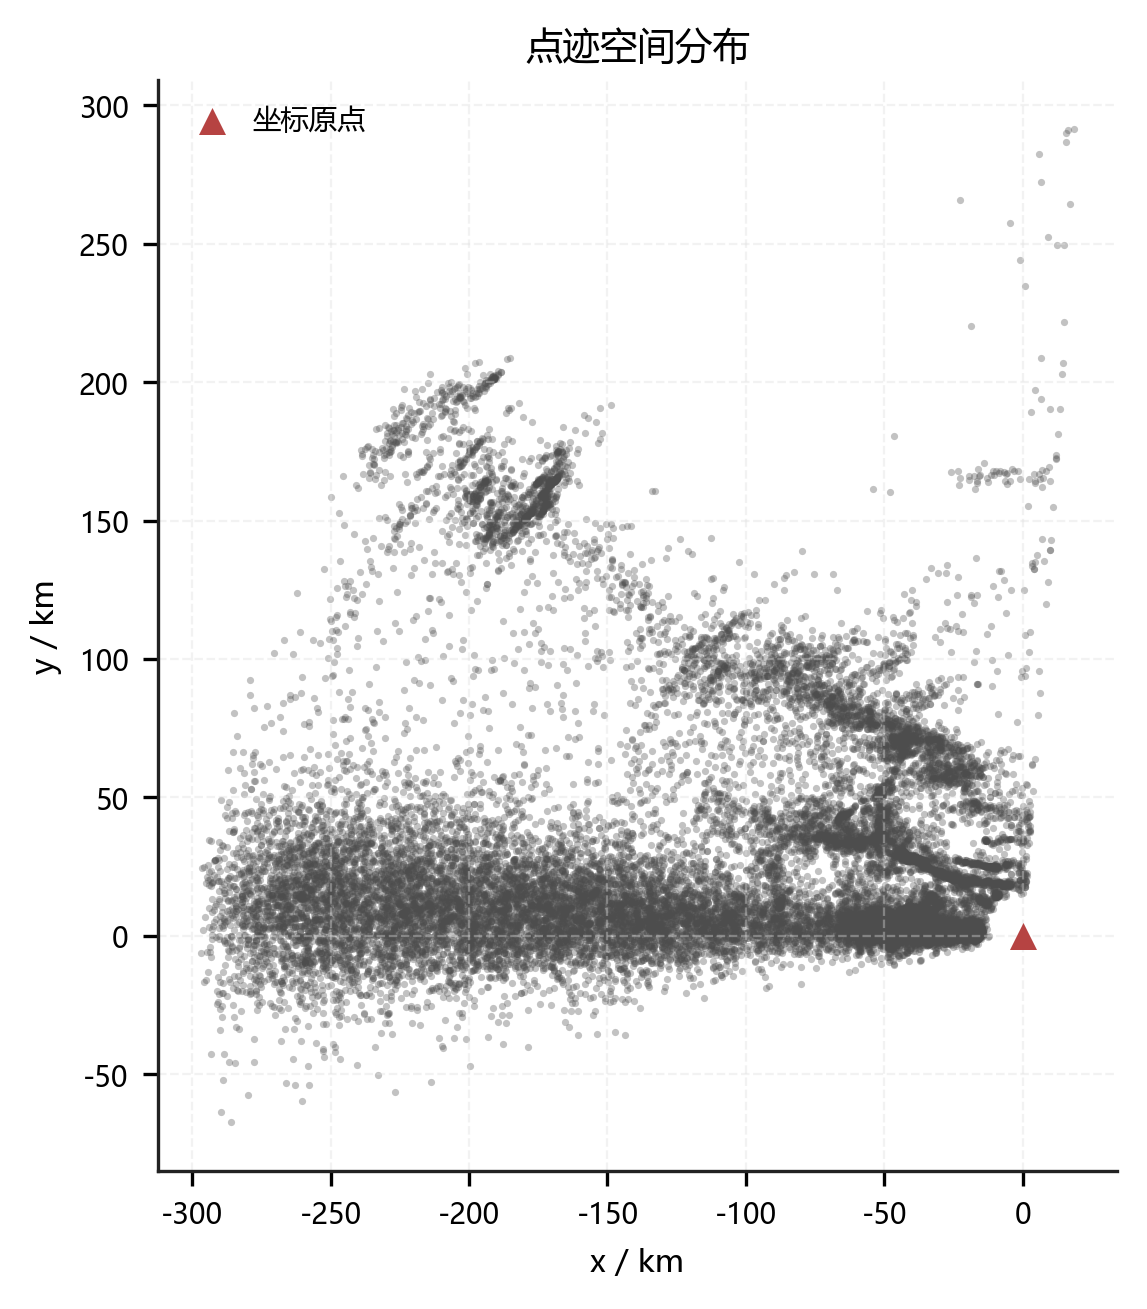
\includegraphics[width=0.72\textwidth]{图2_点迹空间分布.png}
  \caption{全部点迹空间分布}
  \label{fig:spatial_distribution}
\end{figure}

针对图中几个直观上“可能有目标”的区域，本文进一步统计了点迹数、强点比例和候选簇数量，如表 \ref{tab:region_analysis} 所示。结果表明，视觉上较密集的区域确实能够形成单帧候选簇，但这些候选簇并不必然对应稳定目标；只有在多帧关联后仍满足长度、步长和形态质量约束的候选链，才会被保留为疑似目标航迹。

\begin{table}[H]
  \centering
  \caption{典型空间区域候选情况}
  \label{tab:region_analysis}
  \begin{tabular}{lrrrr}
    \toprule
    区域 & 点迹数 & 强点数 & 强点比例 & 候选簇数 \\
    \midrule
    底部长条区域 & 4641 & 423 & 9.1\% & 13 \\
    右中部斜带 & 638 & 375 & 58.8\% & 39 \\
    左上部斑块 & 577 & 382 & 66.2\% & 21 \\
    \bottomrule
  \end{tabular}
\end{table}

表中三个区域分别按平面坐标近似取 \(x\in[-80,5],y\in[0,15]\)、\(x\in[-45,-20],y\in[18,35]\) 和 \(x\in[-72,-50],y\in[32,48]\)，单位均为 km。

\subsubsection{候选检测与确认航迹}

图 \ref{fig:multi_frame_detection} 展示了确认航迹相关帧中的单帧候选检测结果。每帧先保留信号较强点，再通过 DBSCAN 得到候选簇中心。图 \ref{fig:global_tracks} 进一步把全部候选簇中心和最终确认航迹叠加到全局点迹背景上。可以看到，最终确认航迹只占全部点迹空间中的一小部分，这是由多帧连续性和形态质量共同筛选的结果，并不表示其他区域没有点迹。

\begin{figure}[H]
  \centering
  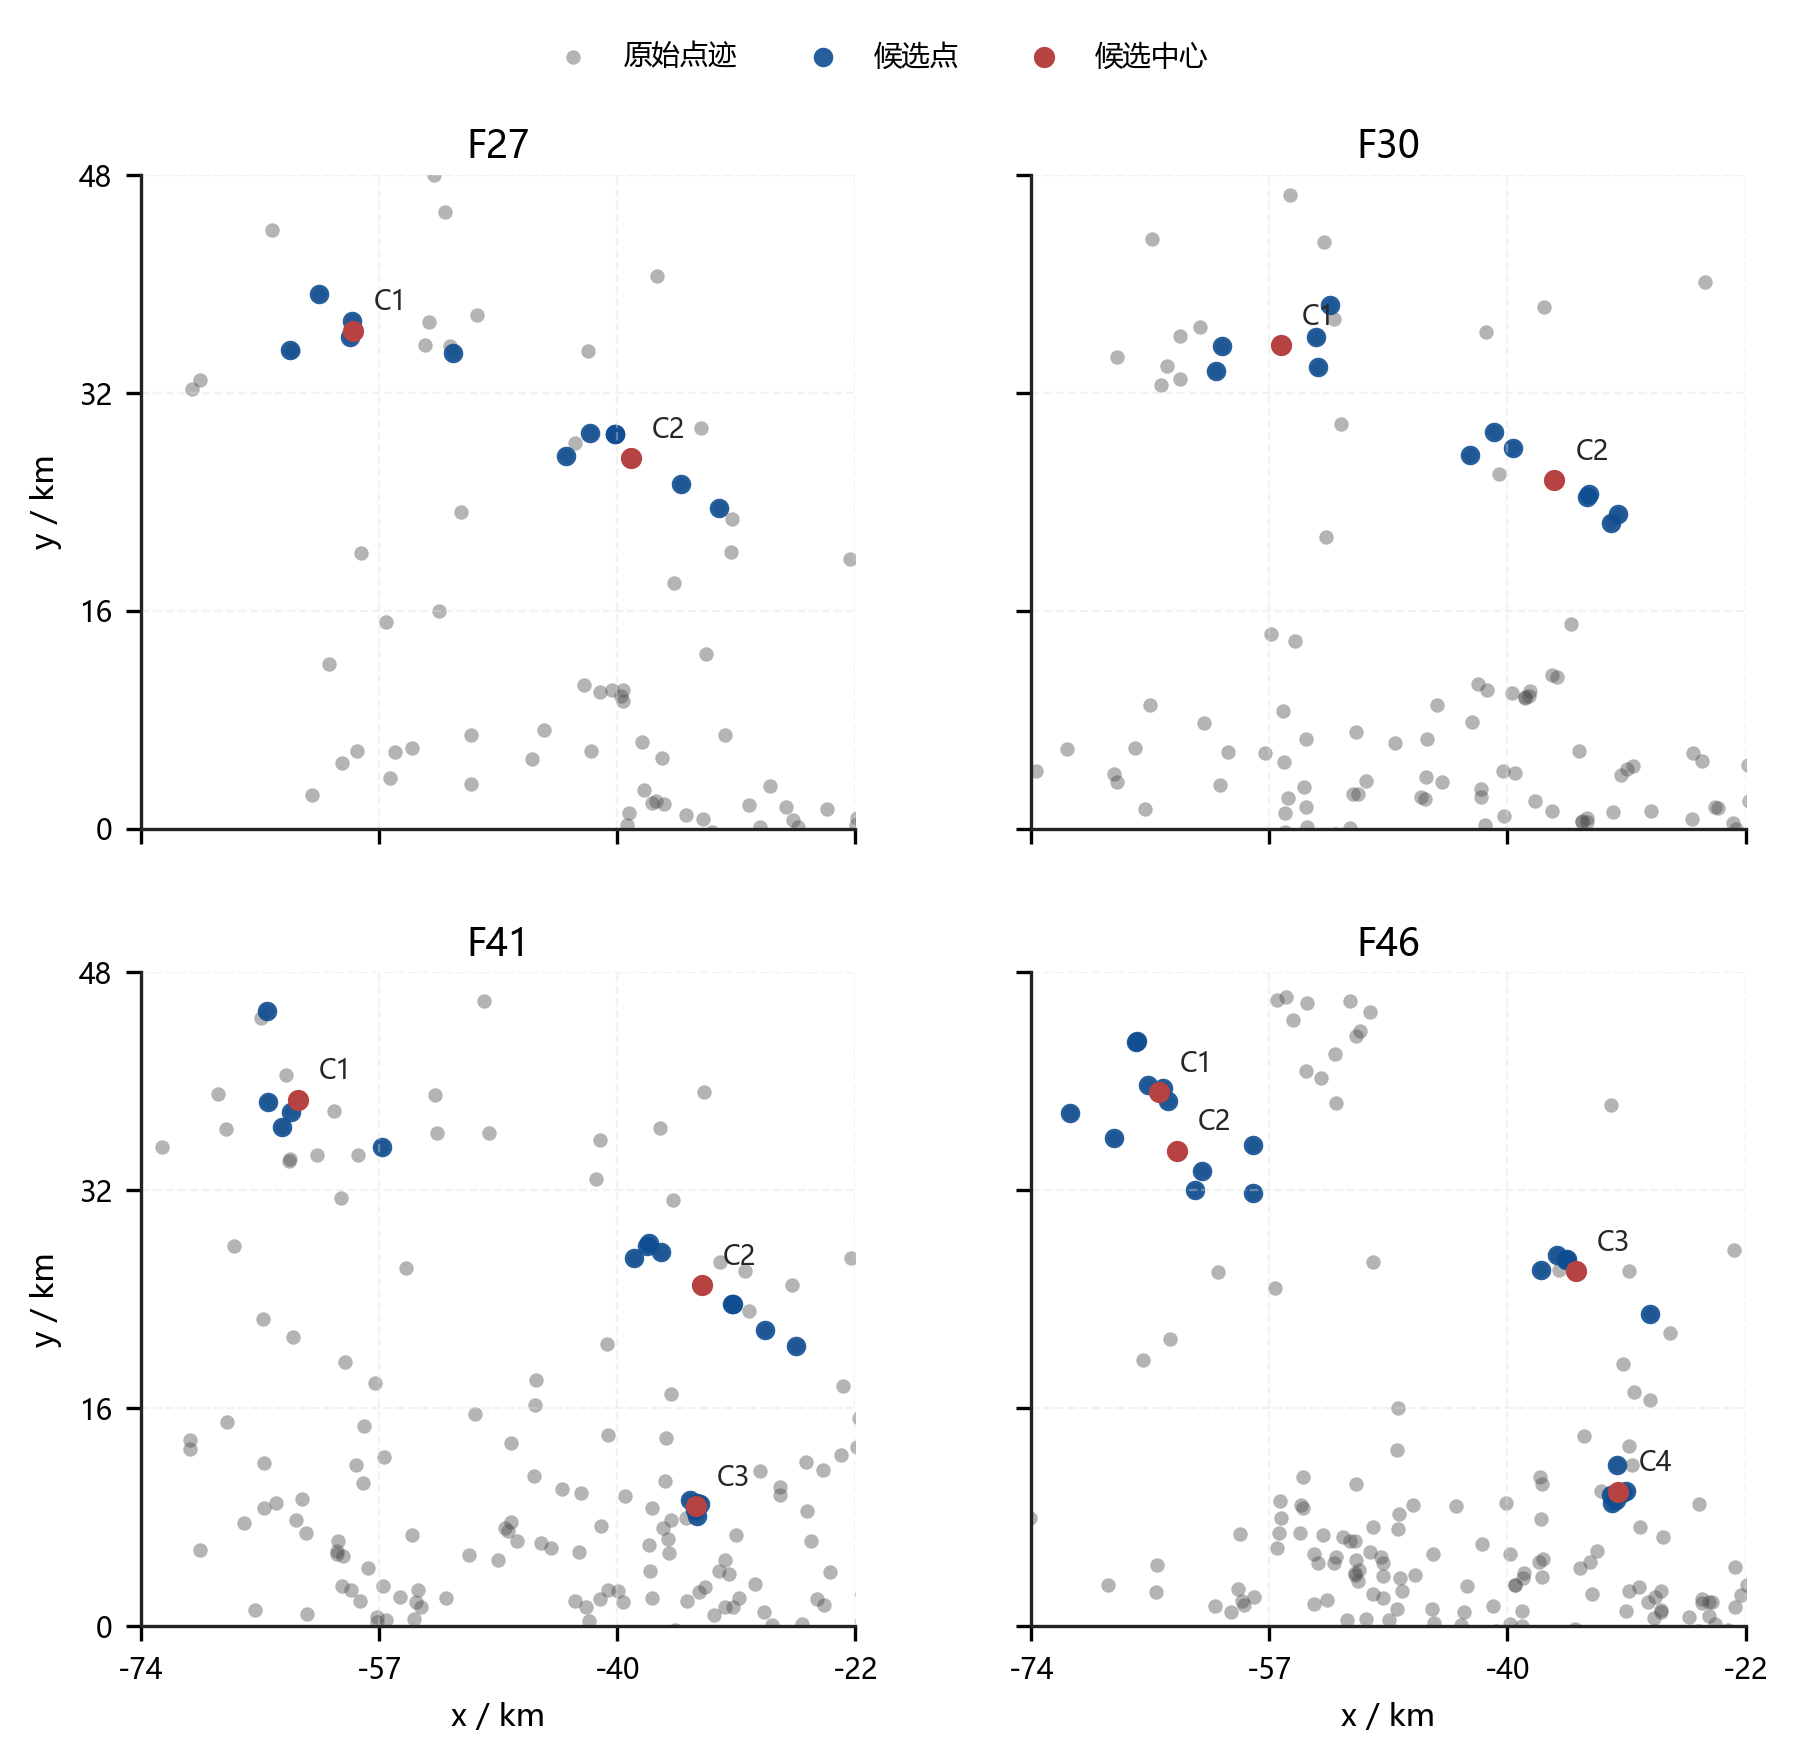
\includegraphics[width=0.92\textwidth]{图3_多帧候选检测.png}
  \caption{多帧候选检测结果}
  \label{fig:multi_frame_detection}
\end{figure}

\begin{figure}[H]
  \centering
  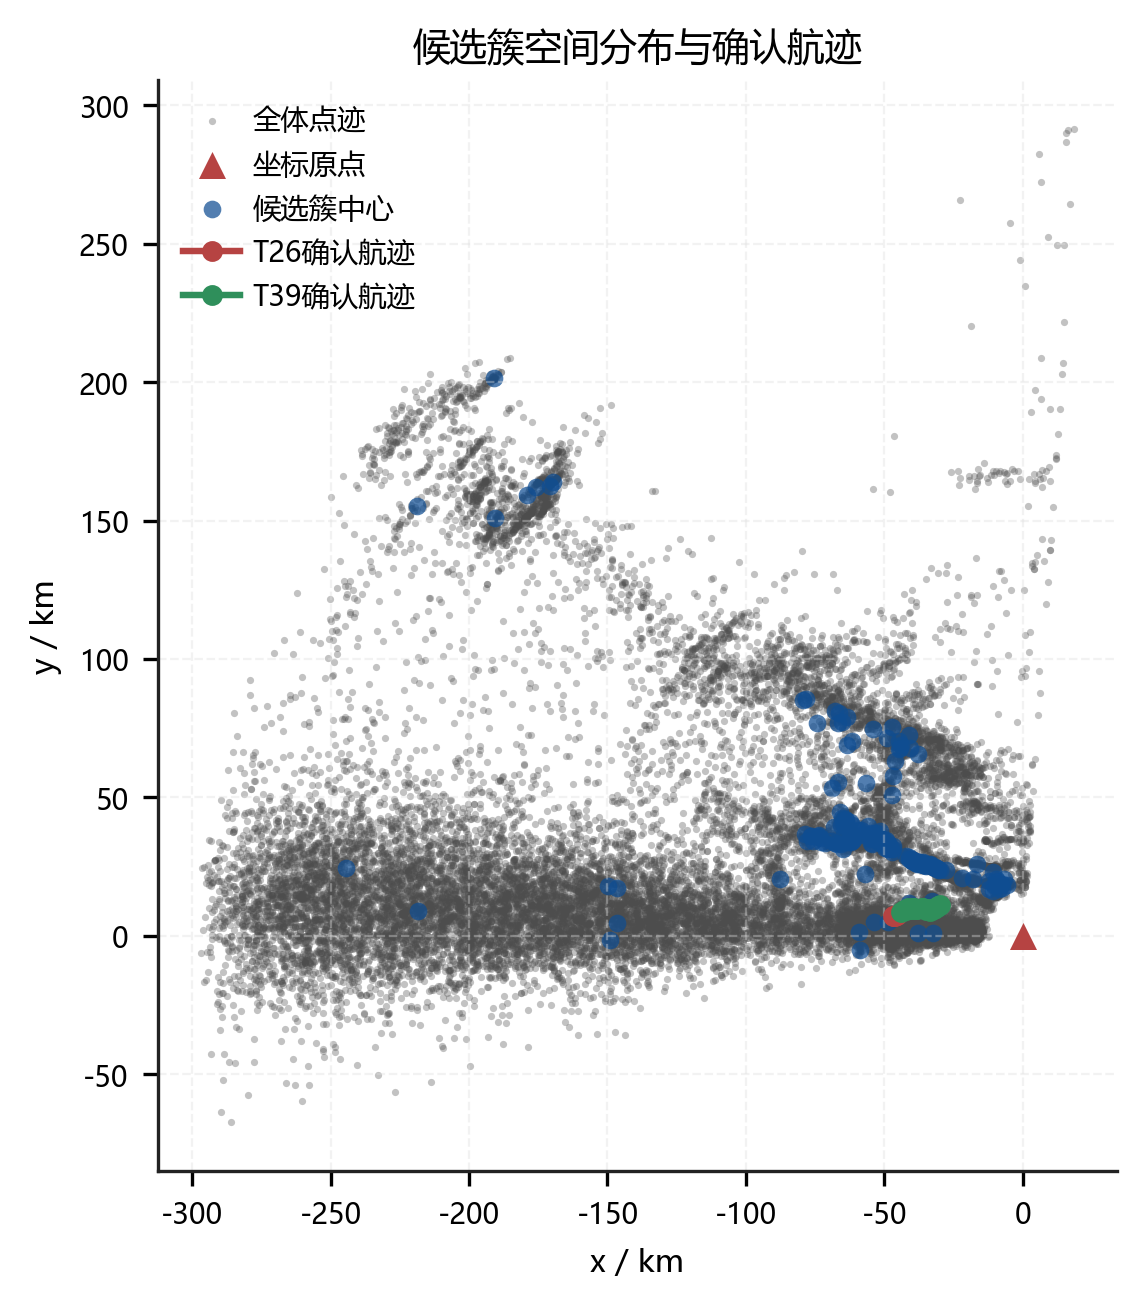
\includegraphics[width=0.72\textwidth]{图4_候选簇与确认航迹.png}
  \caption{候选簇空间分布与确认航迹}
  \label{fig:global_tracks}
\end{figure}

最终确认的两条疑似目标航迹分别为 T25 和 T44。图 \ref{fig:confirmed_tracks} 给出了两条航迹的局部放大结果。T25 出现在第 27--30 帧，持续 4 帧；T44 出现在第 41--46 帧，持续 6 帧。两条航迹均表现出连续中心移动，但 T44 中间存在一定折线变化，因此其直线性低于 T25。

\begin{figure}[H]
  \centering
  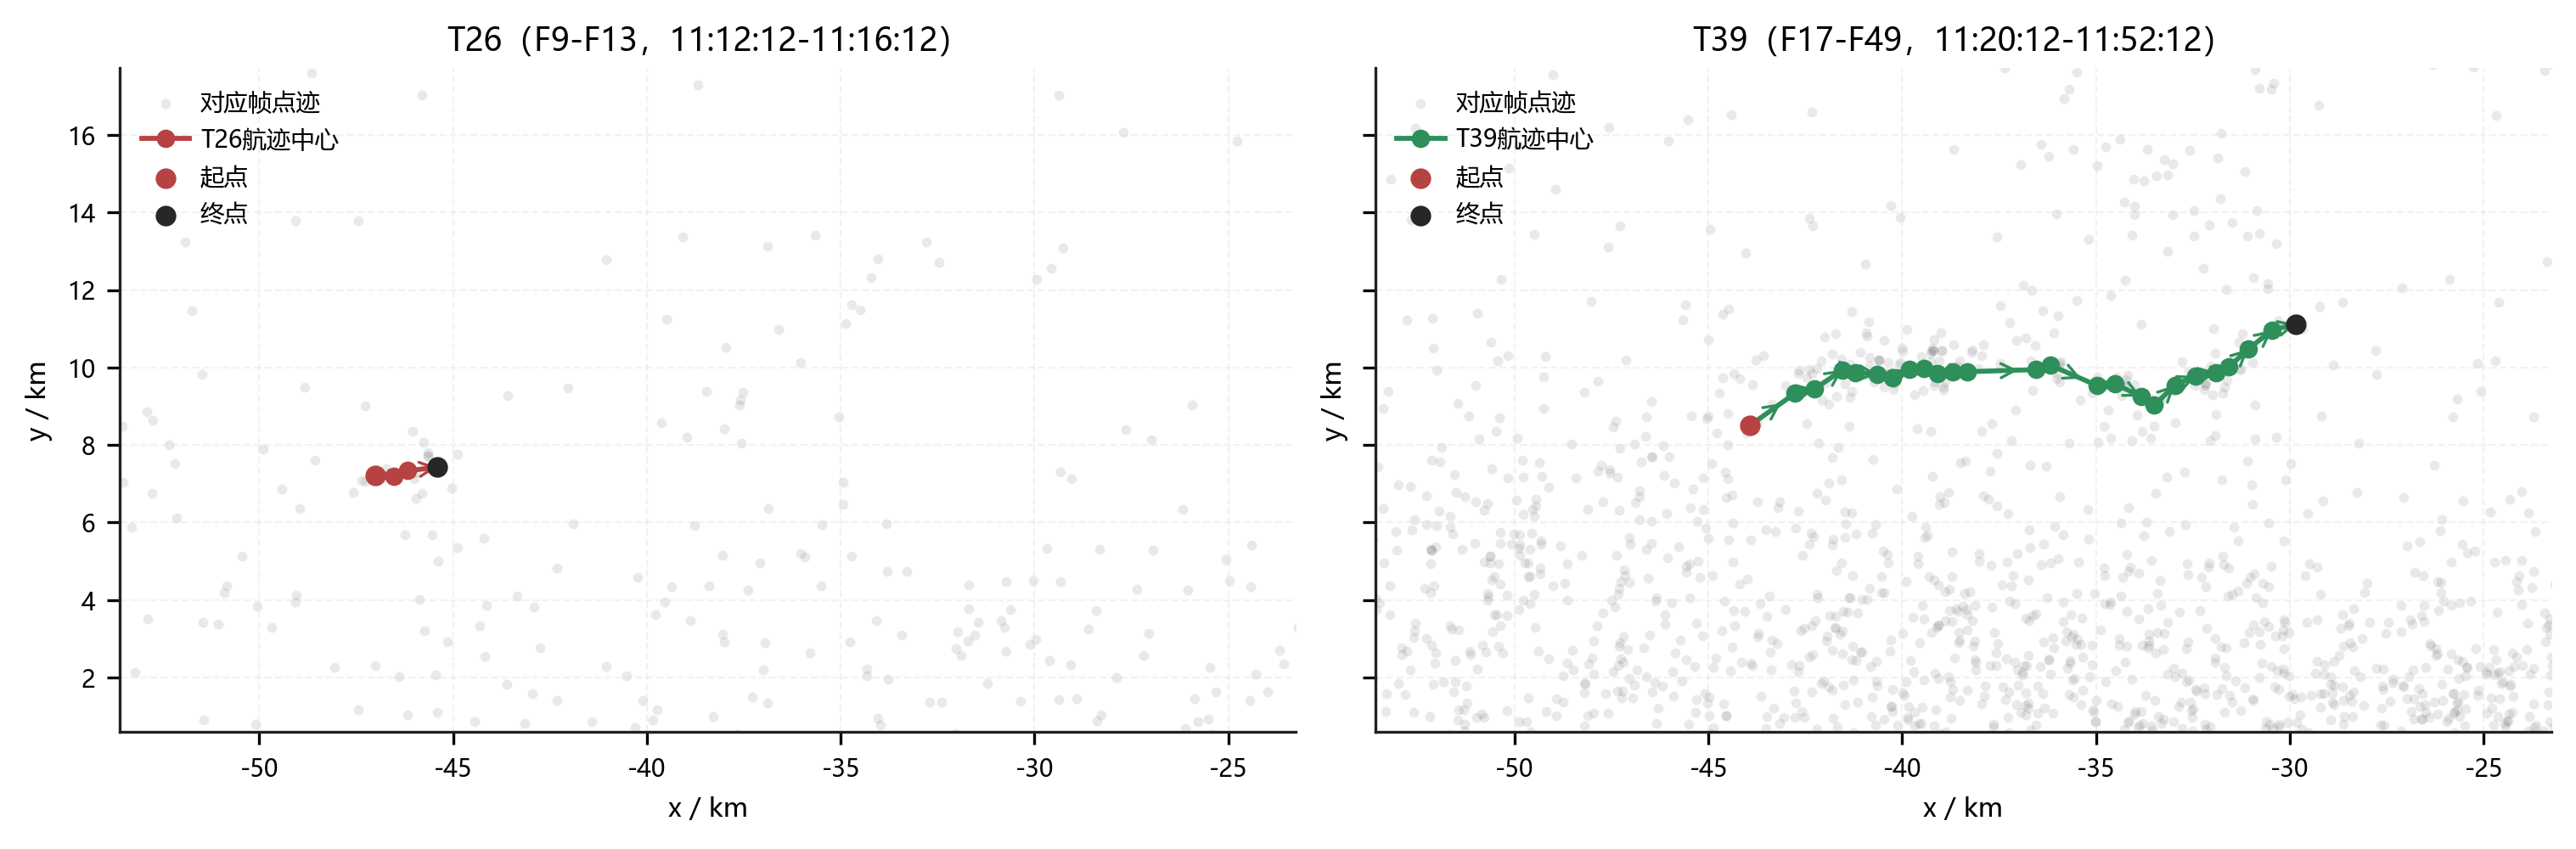
\includegraphics[width=0.96\textwidth]{图5_确认航迹局部放大.png}
  \caption{确认航迹局部放大}
  \label{fig:confirmed_tracks}
\end{figure}

\subsubsection{无监督质量评价}

由于缺少 AIS 或人工标注真值，本文不计算准确率、召回率和 F1 值，而采用无监督质量评价。图 \ref{fig:funnel} 展示了候选筛选数量变化：从 90 个候选簇形成 52 条候选航迹，长度达标航迹为 3 条，最终质量确认航迹为 2 条。图 \ref{fig:quality} 展示了长度达标候选航迹的直线性、步长和最大转向角。

\begin{figure}[H]
  \centering
  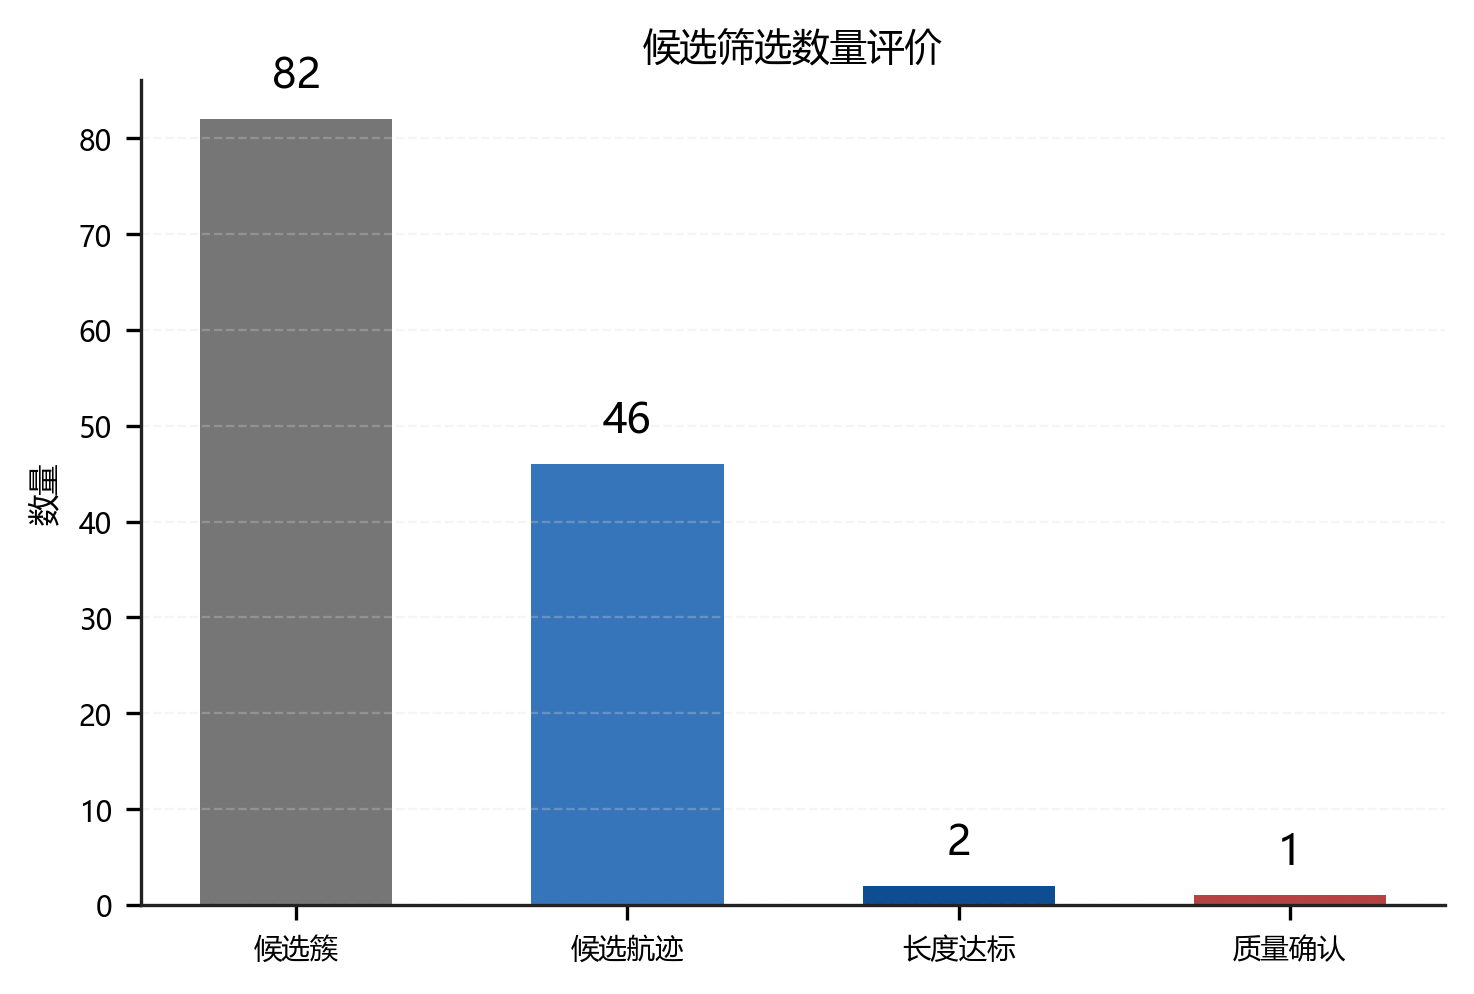
\includegraphics[width=0.62\textwidth]{图6_候选筛选数量评价.png}
  \caption{候选筛选数量变化}
  \label{fig:funnel}
\end{figure}

\begin{figure}[H]
  \centering
  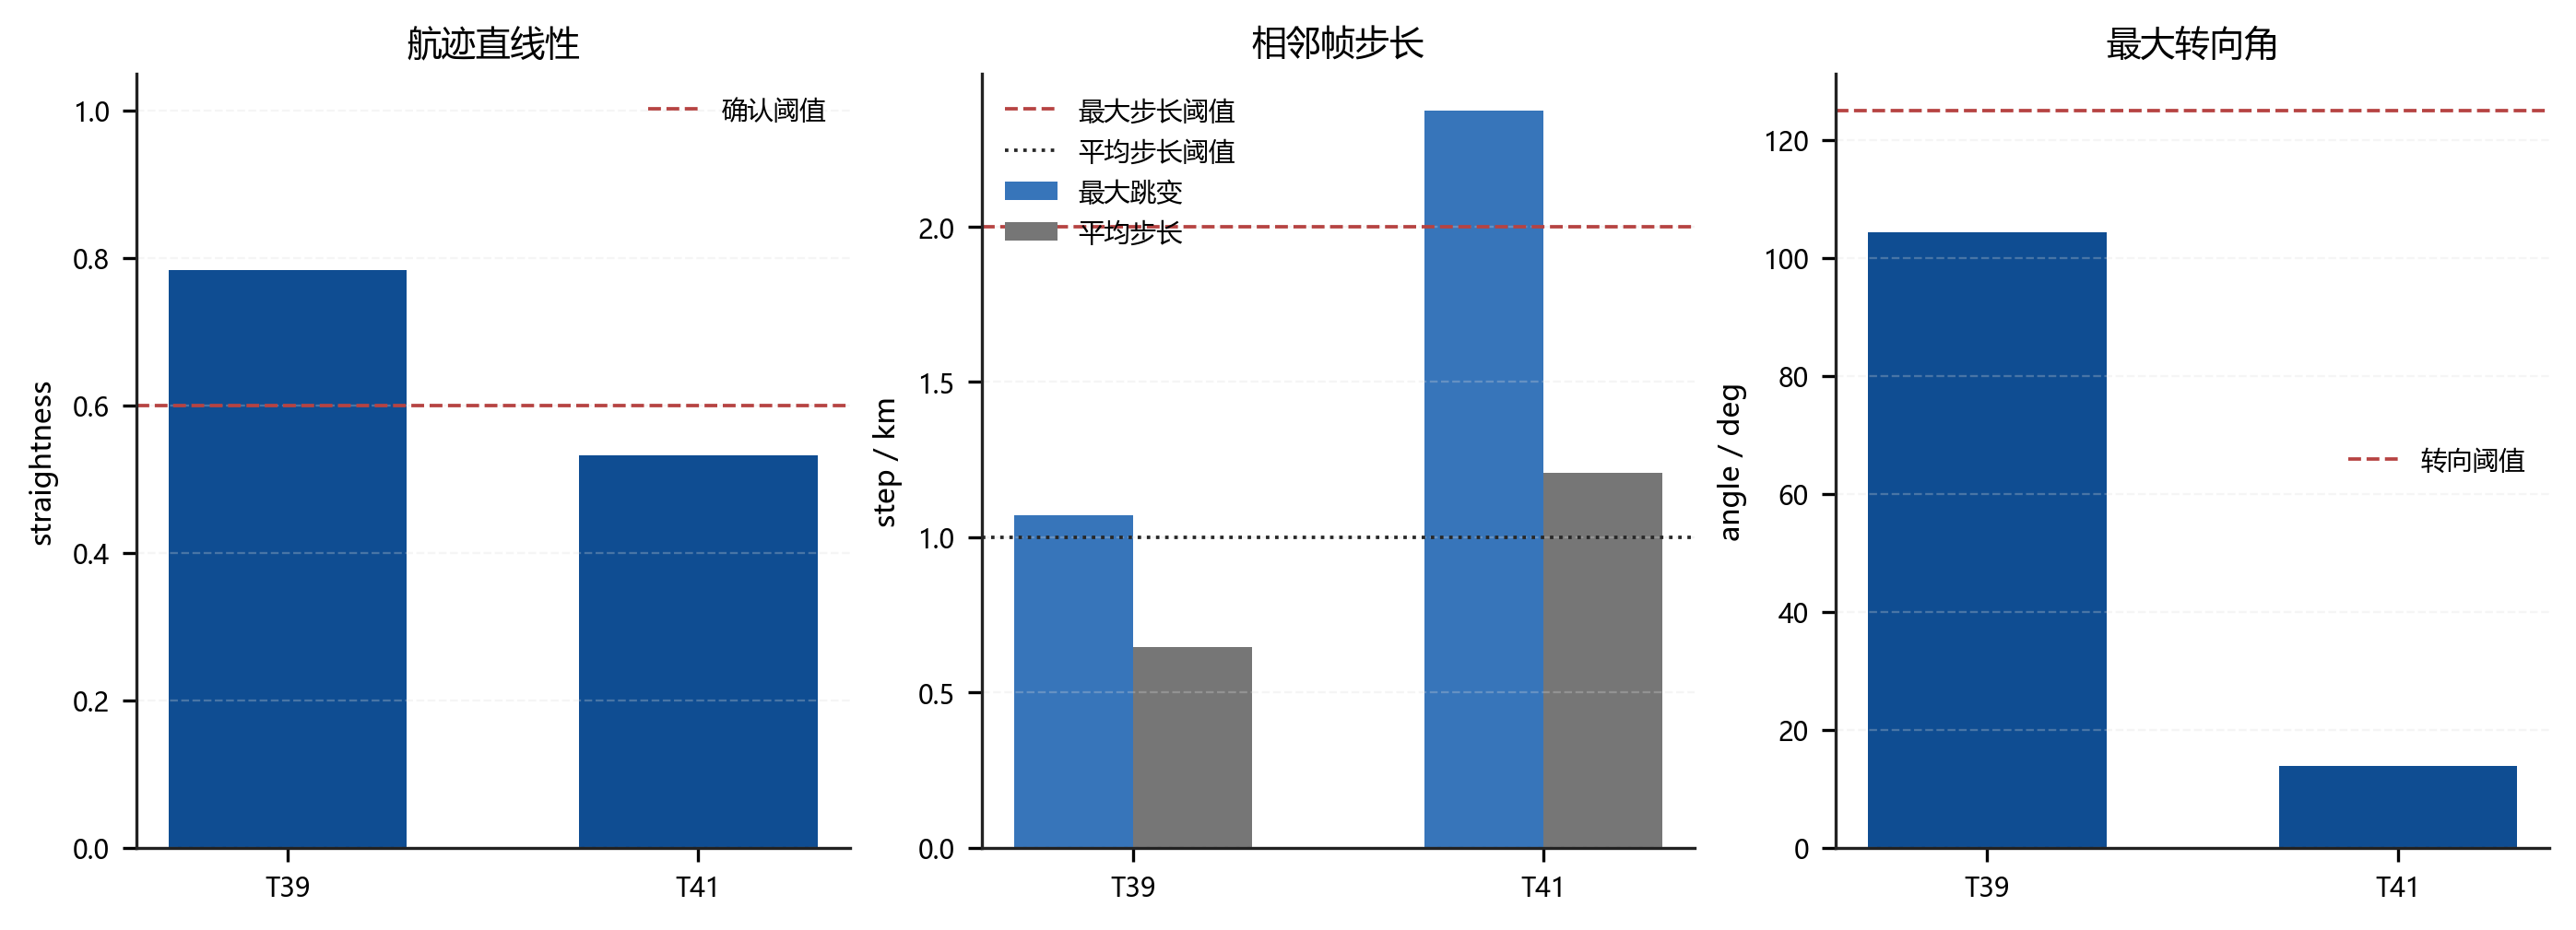
\includegraphics[width=0.92\textwidth]{图7_航迹质量评价.png}
  \caption{航迹质量评价}
  \label{fig:quality}
\end{figure}

\begin{table}[H]
  \centering
  \caption{确认航迹质量摘要}
  \label{tab:track_summary}
  \begin{tabular}{ccccccccc}
    \toprule
    航迹 & 帧数 & 起止帧 & 平均 SNR & 平均速度 & 位移 & 路径长 & 直线性 & 最大步长 \\
    \midrule
    T25 & 4 & F27--F30 & 13.92 & 15.99 & 2.89 & 2.91 & 0.99 & 1.60 \\
    T44 & 6 & F41--F46 & 13.56 & 24.25 & 2.54 & 3.24 & 0.78 & 1.07 \\
    \bottomrule
  \end{tabular}
\end{table}

从表 \ref{tab:track_summary} 可见，T25 的直线性为 0.99，说明其中心点几乎沿单调方向移动；T44 的直线性为 0.78，仍满足质量要求，但存在一定中心抖动。长度达标但未确认的 T46 直线性较低且最大步长偏大，因此更可能是背景点迹被连续关联形成的可疑链，不作为最终确认结果。

\subsubsection{参数敏感性分析}

为评估候选提取条件是否过严或过松，本文比较了三类参数方案。第一类为原始全局强筛选，候选簇数较少，但对弱背景区域不够友好；第二类为直接放松全局阈值，候选数量明显增加，但最近邻关联更容易受到背景候选干扰；第三类为本文最终采用的距离分区补偿方案，候选数量适度增加，同时最终确认航迹数保持稳定。结果如表 \ref{tab:sensitivity} 所示。

\begin{table}[H]
  \centering
  \caption{候选提取参数敏感性分析}
  \label{tab:sensitivity}
  \begin{tabularx}{\textwidth}{lrrrrX}
    \toprule
    方案 & 强点数 & 候选簇 & 候选航迹 & 确认航迹 & 说明 \\
    \midrule
    全局严格筛选 & 2619 & 82 & 46 & 2 & 结果保守，但局部弱区域候选较少 \\
    直接放松阈值 & 5255 & 129 & 79 & 2 & 候选显著增多，误关联风险升高 \\
    距离分区补偿 & 3343 & 90 & 52 & 2 & 适度补充候选，最终结果稳定 \\
    \bottomrule
  \end{tabularx}
\end{table}

该敏感性分析表明，候选提取不能简单地“越宽越好”。如果前端筛选过松，背景点迹会形成大量短寿命候选，反而可能干扰多帧关联；如果过严，则可能完全忽略局部弱信号区域。本文最终方案在候选数量和虚警控制之间取得折中，因此更适合作为课程作业中的可复现实验方案。

\subsubsection{结果边界与方法局限}

本文结果应表述为“疑似目标航迹”或“目标候选”，不能表述为已验证船舶真实航迹。原因在于：第一，本数据没有 AIS 真值或人工标注；第二，当前算法基于点迹后处理，而不是原始距离--多普勒谱上的完整检测；第三，多帧关联采用简化最近邻规则，并未加入完整卡尔曼滤波、概率数据关联或多假设跟踪。

对于图中较宽、较长的灰色点迹带，本文没有直接将其判定为航迹。这是因为这些区域虽然点迹密集，但多数点不满足“高信号、紧凑聚类、多帧连续和平滑移动”的联合条件。后续若需要进一步挖掘弱目标，可考虑引入 track-before-detect、卡尔曼预测门、AIS 对照验证或人工标注样本，以区分真实目标和背景杂波结构。

\section{学习总结与体会}

通过本次大作业，我对高频地波雷达目标探测流程有了更系统的认识。雷达目标检测并不是简单地在散点图上寻找肉眼可见的密集区域，而是需要综合信号强度、空间聚集性、速度一致性和时间连续性。尤其是在点迹背景呈现宽带状和斑块状分布时，直观密集区域并不一定对应稳定目标；只有能够在相邻帧中连续出现并满足物理约束的候选链，才更适合被保留为疑似航迹。

本实验也说明，参数选择需要在漏检和虚警之间折中。过严的信噪比和幅度筛选会忽略局部弱信号区域，过松的筛选又会造成候选簇数量膨胀并增加误关联。通过敏感性分析可以看到，距离分区补偿比简单放松全局阈值更稳健，能够适当补充候选而不破坏最终质量确认结果。

在方法边界方面，本文没有将结果包装成“准确率”或“真实目标确认”，而是采用无监督质量指标解释结果。这一点对雷达数据分析非常重要：当没有 AIS 或人工标注作为真值时，算法输出只能说明候选链在当前规则下满足连续性和形态质量，不能证明其一定是船舶目标。后续若继续改进，可将卡尔曼滤波、概率数据关联、AIS 验证和原始谱级检测结合起来，使目标跟踪结果更接近工程应用要求。

\end{document}
